\documentclass[10pt]{beamer}


\usepackage{amsmath}
\usepackage{amstext}
\usepackage{amsfonts}
\usepackage{amssymb}
\usepackage{array}
\usepackage{graphicx}
\usepackage{slashed}
\usepackage{color}
\usepackage{epstopdf}
\usepackage{caption}
\usepackage{multirow}
\usepackage{overpic}
\usepackage{tikz}
\usepackage{animate}
\usetikzlibrary{shapes.callouts}
\usetikzlibrary{decorations.text}
\usetikzlibrary{decorations.pathreplacing}
\usetikzlibrary{arrows,shapes,shadows}
\usetikzlibrary{calc}
\usetikzlibrary{backgrounds}

\DeclareMathOperator{\mean}{mean}

\beamertemplatenavigationsymbolsempty
\usetheme{Boadilla}
\definecolor{FERMILABblue}{RGB}{65,182,230}% FERMILAB 
\usecolortheme[RGB={0,76,151}]{structure} %FERMILAB
\setbeamertemplate{frametitle}[default][center]
\usepackage{textcomp}




\title[Machine Learning Phase Space]{Improving Numerical Integration and Event Generation with Normalizing Flows}
\subtitle{ --- HET Brown Bag Seminar, University of Michigan ---}
\author[Claudius Krause]{\large Claudius Krause}
\date{September 25, 2019}
\institute[Fermilab]{Fermi National Accelerator Laboratory}
\titlegraphic{\vspace*{-0.5cm}\includegraphics[height=1cm]{Logo/FNAL-Logo-NAL-Blue.pdf} \hspace{1.5cm}\includegraphics[height=2cm,trim=0 50 0 50,clip]{Logo/Humboldt-Stiftung.jpg} }

\begin{document}


% Slide 1 (title)
\begin{frame}
  \titlepage
  \begin{scriptsize}
    \begin{center}
      In collaboration with: Christina Gao, Stefan H\"oche, Joshua Isaacson\\
      arXiv: 191x.abcde
    \end{center}
  \end{scriptsize}
\end{frame}


% Slide 2 (motivation)
\begin{frame}
  \frametitle{Monte Carlo Simulations are increasingly important.}
  \vspace*{-0.5em}
  \tikzstyle{blockgr} = [draw, text width=32em, fill=FERMILABblue!20, rounded corners, drop shadow]
  \begin{center}
    \begin{tikzpicture}
      \node (pic) [text width = 0.8\textwidth, text centered] at (0em,0em) {\includegraphics[width=0.925\textwidth]{figures/cpuHLLHC_noold.png}};
      \node (ref) [text width = 30em,anchor = south, text centered] at ($(pic.south)+(0em,-0.75em)$){\begin{scriptsize}\textcolor[rgb]{.4,.4,.4}{https://twiki.cern.ch/twiki/bin/view/AtlasPublic/ComputingandSoftwarePublicResults}\end{scriptsize}};      
      \node at ($(pic.south)+(0em,-2.5em)$) (text) [blockgr] {
        \begin{itemize}
        \item[$\Rightarrow$] MC event generation is needed for signal and background predictions.
        \item[$\Rightarrow$] The required CPU time will increase in the next years. 
        \end{itemize}
      };
    \end{tikzpicture}
  \end{center}
\end{frame}


% Slide 3 (motivation)
\begin{frame}
  \frametitle{Monte Carlo Simulations are increasingly important.}
  \vspace*{-2em}
  \tikzstyle{blockgr} = [draw, text width=30em, fill=FERMILABblue!20, rounded corners, drop shadow]
  \begin{center}
    \begin{tikzpicture}
      \node (pic) [text width = \textwidth, text centered] at (0em,0em) {\includegraphics[width=0.48\textwidth]{source/1905.05120/fig/timing.pdf}\hfill \includegraphics[width=0.48\textwidth]{source/1905.05120/fig/wpj/trials.pdf}};
      \node (ref) [text width = 30em,anchor = south, text centered] at ($(pic.south)+(0em,-0.75em)$){\begin{scriptsize}\textcolor[rgb]{.4,.4,.4}{Stefan H\"oche, Stefan Prestel, Holger Schulz [1905.05120;PRD]}\end{scriptsize}};      
      \node at ($(pic.south)+(0em,-5em)$) (text) [blockgr] {
        The bottlenecks for evaluating large final state multiplicities are \\
        $ $ 
        \begin{itemize}
        \item a slow evaluation of the matrix element
        \item a low unweighting efficiency
        \end{itemize}
      };
      \uncover<2>{\draw ($(text.south)+(-8em,0.75em)$) ellipse (8em and 1.5em);}
    \end{tikzpicture}
  \end{center}
\end{frame}


% Slide 4 (Mapping)
\begin{frame}
  \frametitle{Improving Numerical Integration and Event Generation with Normalizing Flows}
  \vspace{0.5cm}
  \tikzstyle{part} = [text width = 8cm]
  \begin{tikzpicture}
    \node [part, align = right, text width = 8cm](part1) at (-5em,0em) {\large Part I: \quad The ``traditional'' approach};
    \node [anchor = west](part1pic) at ($(part1.north east)+(1.5em,-0.75em)$) {\framebox{\includegraphics[width=8em]{figures/VEGAS_grid.pdf}}};
    \node [part, align = right, text width=9cm](part2) at (4em,-8em) {\large Part II: \quad  The Machine Learning approach};
    \node [anchor = east] (part2pic) at ($(part2.north west)+(4em,-0.75em)$) {\framebox{\includegraphics[width=8em,trim = 30 20 10 10,clip]{figures/NN.pdf}}};
  \end{tikzpicture}
\end{frame}


\section{Part I: \quad The ``traditional'' approach}


% Slide 5
\begin{frame}
  \frametitle{\vspace{-0.85cm}\begin{columns}\column{0.1\textwidth}\framebox{\includegraphics[width=\textwidth]{figures/VEGAS_grid.pdf}}\column{0.85\textwidth}\vspace{-0.2cm}I: There are two problems to be solved\dots\end{columns}}
  \tikzstyle{block} = [draw, text width=32em, fill=FERMILABblue!20, rounded corners, drop shadow, minimum height = 2em, text centered]
  \vspace*{-2em}
  \begin{center}
    \begin{tikzpicture}
      \node (problem1) [block] at (0,0) {\vspace*{-1em}\begin{align}\begin{aligned}\nonumber f(\vec{x})\quad &\uncover<2->{\Rightarrow \quad F = \int f(\vec{x})\; d^{D}x}\\
            d\sigma(p_{i},\vartheta_{i},\varphi_{i}) \quad &\uncover<2->{\Rightarrow \quad \sigma = \int d\sigma(p_{i},\vartheta_{i},\varphi_{i}), \quad D= 3n_{\text{final}} -4}\end{aligned}\end{align}
      };
      \uncover<3->{
        \node (problem2) [block,anchor=north] at ($(problem1.south)+(0em,-1em)$) {Given a distribution $f(\vec{x})$, how can we sample according to it?}; 
      }
      \node (plot0) [anchor=north, text width = 15em] at ($(problem2.south)+(-7.5em,-0.5em)$) {\includegraphics[width=0.75\textwidth]{figures/pdf.pdf}};
      \uncover<2>{
        \node (plot1) [anchor=west, text width = 15em] at ($(plot0.east)+(4em,0em)$) {\includegraphics[width=0.75\textwidth]{figures/pdf_filled.pdf}};
      }
      \uncover<2->{\node (arrow) [anchor = west, text width = 4em, text centered] at ($(plot0.east)+(-2em,0em)$) {\begin{Large}?\\$\Longrightarrow$\end{Large}};}
      \uncover<3>{
        \node (plot2) [anchor=west, text width = 15em] at ($(plot0.east)+(4em,0em)$) {\includegraphics[width=0.75\textwidth]{figures/pdf_sampled.pdf}};
      }
    \end{tikzpicture}
  \end{center}
\end{frame}


% Slide 6 
\begin{frame}
  \frametitle{\vspace{-0.85cm}\begin{columns}\column{0.1\textwidth}\framebox{\includegraphics[width=\textwidth]{figures/VEGAS_grid.pdf}}\column{0.85\textwidth}\vspace{-0.2cm}I: \dots but they are closely related.\end{columns}}
  \tikzstyle{block} = [draw, text width=32em, fill=FERMILABblue!20, rounded corners, drop shadow, minimum height = 2em, text centered]
  \vspace*{-2em}
  \begin{center}
    \begin{tikzpicture}
      \node (problem1) [block] at (0,0) {\begin{enumerate}
        \item Starting from a pdf, \dots
        \item \dots we can integrate it and find its cdf, \dots
        \item \dots to finally use its inverse to transform a uniform distribution.
        \end{enumerate}
      };
      \node (plot0) [anchor=north, text width = 10em] at ($(problem1.south)+(-10.5em,-1.5em)$) {\includegraphics[width=0.75\textwidth]{figures/pdf.pdf}};
      \node (arrow1) [anchor = west,text width = 2em] at ($(plot0.east)+(-1.5em,0em)$) {$\Rightarrow$};
      \node (number1) [anchor = south, text width = 2em, text centered] at ($(plot0.north west)+(0em,-1em)$) {\begin{enumerate} \item $ $ \end{enumerate}
      };
      \node (plot1) [anchor=west, text width = 10em] at ($(plot0.east)+(1em,0em)$) {\includegraphics[width=0.75\textwidth]{figures/cdf.pdf}};
      \node (arrow2) [anchor = west,text width = 2em] at ($(plot1.east)+(-1.5em,0em)$) {$\Rightarrow$};
      \node (number2) [anchor = south, text width = 2em, text centered] at ($(plot1.north west)+(0em,-1em)$) {\begin{enumerate}\setcounter{enumi}{1} \item $ $ \end{enumerate}
      };
      \node (plot2) [anchor=west, text width = 10em] at ($(plot1.east)+(1em,0em)$) {\includegraphics[width=0.75\textwidth]{figures/invcdf.pdf}};
      \node (number3) [anchor = south, text width = 2em, text centered] at ($(plot2.north west)+(0em,-1em)$) {\begin{enumerate}\setcounter{enumi}{2} \item $ $ \end{enumerate}
      };
      \uncover<2->{
        \node (text) [anchor = north, block, text centered] at ($(problem1.south)+(0em,-10em)$) {$\Rightarrow $ We need a fast and effective numerical integration!};
      }
    \end{tikzpicture}
  \end{center}
\end{frame}


% Slide 7 
\begin{frame}
  \frametitle{\vspace{-0.85cm}\begin{columns}\column{0.1\textwidth}\framebox{\includegraphics[width=\textwidth]{figures/VEGAS_grid.pdf}}\column{0.85\textwidth}\vspace{-0.2cm}I: Importance Sampling is very efficient for high-dimensional integration.\end{columns}}
  \tikzstyle{block} = [draw, text width=32em, fill=FERMILABblue!20, rounded corners, drop shadow, minimum height = 2em, text centered]
  \vspace*{-2em}
  \begin{center}
    \begin{tikzpicture}
      \node (MC) [block] at (0,0) {\vspace*{-1em} $$\int_{0}^{1} f(x)\; dx \qquad \xrightarrow{\text{MC}}\qquad \frac{1}{N} \sum_{i} f(x_{i})\qquad x_{i}\dots \text{uniform}$$
      };
      \node (MCimp) [anchor = north, block] at ($(MC.south)+(0em,-2em)$) {$$=\int_{0}^{1} \frac{f(x)}{q(x)}\; q(x)dx \qquad \xrightarrow[\text{importance sampling}]{\text{MC}}\qquad \frac{1}{N} \sum_{i} \frac{f(x_{i})}{q(x_{i})}\qquad x_{i}\dots q(x)$$};
      \uncover<2->{
        \node (bottomline) [anchor = north, block] at ($(MCimp.south)+(0em,-2em)$) {We therefore have to find a $q(x)$ that
          \begin{itemize}
          \item approximates the shape of $f(x)$.
          \item is ``easy'' enough such that we can sample from its inverse cdf.
          \end{itemize}
        };
      }
    \end{tikzpicture}
  \end{center}
\end{frame}


% Slide 8 
\begin{frame}
  \frametitle{\vspace{-0.85cm}\begin{columns}\column{0.1\textwidth}\framebox{\includegraphics[width=\textwidth]{figures/VEGAS_grid.pdf}}\column{0.85\textwidth}\vspace{-0.2cm}I: The unweighting efficiency measures the quality of the approximation $q(x)$.\end{columns}}
  \tikzstyle{block} = [draw, text width=32em, fill=FERMILABblue!20, rounded corners, drop shadow, minimum height = 2em, text centered]
  \vspace*{-2em}
  \begin{center}
    \begin{tikzpicture}
      \node (uniform) [block] at (0,0) {
        \begin{itemize}
        \item If $q(x)$ were constant, each event $x_{i}$ would require a weight of $f(x_{i})$ to reproduce the distribution of $f(x)$. $\quad\qquad\qquad\Rightarrow$ ``Weighted Events''
        \item[$ $]
        \item To unweight, we need to accept/reject each event with probability $\frac{f(x_{i})}{\max{f(x)}}$. The resulting set of kept events is unweighted and reproduces the shape of $f(x)$.
        \end{itemize}
      };
      \uncover<2->{
        \node (likef) [block,anchor=north] at ($(uniform.south)+(0em,-1em)$) {
          \begin{itemize}
          \item If $q(x)\propto f(x)$, all events would have the same weight as the distribution reproduces $f(x)$ directly. 
          \end{itemize}
        };
      }
      \uncover<3->{
        \node (def) [block,anchor=north, align=left] at ($(likef.south)+(0em,-1em)$) {We define the $\qquad\qquad$\framebox{Unweighting Efficiency $ = \frac{\# \text{ accepted events}}{\# \text{ all events}} = \frac{\mean{w}}{\max{w}}$}, \\ with $w_{i} = \frac{p(x_{i})}{q(x_{i})} = \frac{f(x_{i})}{F q(x_{i})}$.
        };
      }
    \end{tikzpicture}
  \end{center}
\end{frame}


% Slide 9
\begin{frame}
  \frametitle{\vspace{-0.85cm}\begin{columns}\column{0.1\textwidth}\framebox{\includegraphics[width=\textwidth]{figures/VEGAS_grid.pdf}}\column{0.85\textwidth}\vspace{-0.2cm}I: The {\tt VEGAS} algorithm is very efficient.\end{columns}}
  \tikzstyle{block} = [draw, text width=32em, fill=FERMILABblue!20, rounded corners, drop shadow, minimum height = 2em, text centered]
  \vspace*{-2em}
  \begin{center}
    \begin{tikzpicture}
      \node (vegas) [block,minimum height = 10em] at (0,0) {The {\tt VEGAS} algorithm\\
        \begin{itemize}
        \item assumes the integrand factorizes and bins the 1-dim projection.
        \item then adapts the bin edges such that area of each bin is the same.
        \item[$ $]
        \item[$ $]
        \item[$ $]
        \item[$ $]
        \item[$ $]
        \end{itemize}
      };
      \node (ref) [anchor = north east, text width = 15em, align = right] at ($(vegas.north east)$) {\begin{scriptsize} \textcolor[rgb]{.4,.4,.4}{Peter Lepage 1980} \end{scriptsize}};
      \node (plot0) [anchor=south, text width = 6em] at ($(vegas.south)+(-5em,0.5em)$) {\includegraphics[width=\textwidth]{figures/VEGAS_start.pdf}};
      \node (plot1) [anchor=west, text width = 6em] at ($(plot0.east)+(4em,0em)$) {\includegraphics[width=\textwidth]{figures/VEGAS_grid.pdf}};
      \node (arrow) [anchor = west, text width = 4em, text centered] at ($(plot0.east)+(0em,0em)$) {\begin{Large}$\Longrightarrow$\end{Large}};
      \uncover<2->{
        \node (problems) [block,anchor=north,minimum height = 8em] at ($(vegas.south)+(0em,-1em)$) {
          \begin{itemize}
          \item It does have problems if the features are \\ not aligned with the coordinate axes.
          \item The current {\tt python} implementation also uses \\ stratified sampling.
          \end{itemize}
        };
        \node (probpic) [anchor=south east, text width = 8em] at ($(problems.south east)+(0em,0em)$) {\includegraphics[width=\textwidth]{figures/VEGAS_camel.pdf}};
      }
    \end{tikzpicture}
  \end{center}
\end{frame}


% Slide 10  (Mapping)
\begin{frame}
  \frametitle{Improving Numerical Integration and Event Generation with Normalizing Flows}
  \vspace{0.5cm}
  \tikzstyle{part} = [text width = 8cm]
  \begin{tikzpicture}
    \node [part, align = right, text width = 8cm](part1) at (-5em,0em) {\large Part I: \quad The ``traditional'' approach};
    \node [anchor = west](part1pic) at ($(part1.north east)+(1.5em,-0.75em)$) {\framebox{\includegraphics[width=8em]{figures/VEGAS_grid.pdf}}};
    \node [part, align = right, text width=9cm](part2) at (4em,-8em) {\large Part II: \quad  The Machine Learning approach};
    \node [anchor = east] (part2pic) at ($(part2.north west)+(4em,-0.75em)$) {\framebox{\includegraphics[width=8em,trim = 30 20 10 10,clip]{figures/NN.pdf}}};
  \end{tikzpicture}
\end{frame}


\section{Part II: \quad The Machine Learning approach}


% Slide  11 (Sub-Mapping)
\begin{frame}
  \frametitle{Part II: \quad The Machine Learning approach}
  \vspace{0.5cm}
  \tikzstyle{partR} = [text width = 7cm,align=right]
  \tikzstyle{partL} = [text width = 7cm,align=left]
  \hspace*{-3em}
  \begin{tikzpicture}
    \node [partL](part1) at (0em,0em) {\large Part II.1: \quad Neural Network Basics};
    \node [anchor = west, text width = 6em](part1pic) at ($(part1.north east)+(1.5em,-0.75em)$) {\framebox{\includegraphics[width=8em,trim = 30 20 10 10,clip]{figures/NN.pdf}}};
    
    \node [partL, text width=20em,anchor=north] (part2) at ($(part1pic.south)+(0em,-3em)$) {\large Part II.2: \quad  Numerical Integration \\ with Neural Networks};
    \node [anchor = east, text width = 15em,align=left] (part2pic) at ($(part2.north west)+(0em,-0.75em)$) {\framebox{\includegraphics[width=14em]{figures/CL.png}}};

    \node [partL, align = right, text width = 8cm,anchor = north](part3) at ($(part2pic.south) + (0em,-4em)$) {\large Part II.3: \quad Examples};
    \node [anchor = west](part1pic) at ($(part3.north east)+(1.5em,-0.75em)$) {\framebox{\includegraphics[width=8em]{figures/3j_kin.png}}};
  \end{tikzpicture}
\end{frame}


\subsection{Part II.1: \quad Neural Network Basics}


% Slide 12 
\begin{frame}
  \frametitle{\vspace{-0.85cm}\begin{columns}\column{0.1\textwidth}\framebox{\includegraphics[width=\textwidth,trim = 30 20 10 10,clip]{figures/NN.pdf}}\column{0.85\textwidth}\vspace{-0.2cm}II.1: Neural Networks are nonlinear functions, inspired by the human brain.\end{columns}}
  \tikzstyle{block} = [draw, text width=32em, fill=FERMILABblue!20, rounded corners, drop shadow, minimum height = 8em, text centered]
  \vspace*{-1.75em}
  \begin{center}
    \begin{tikzpicture}
      \node (NN) [block] at (0,0) {Each neuron transforms the input with a weight $W$ and a bias $\vec{b}$. \\ $ $\\
        \begin{tikzpicture}[background rectangle/.style={fill=white}, show background rectangle]
          \node (eq) [text width = 12.5em, minimum height = 7.5em] at (0,0) {$W \vec{x} +\vec{b} $};
          \draw (0,0) circle (2.5em);
          \draw[thick,->] ($(-6em,0em)$) -- ($(-2.5em,0em)$);
          \draw[thick,->] ($(-6em,3em)$) -- ($(-2.165em,1.25em)$);
          \draw[thick,->] ($(-6em,-3em)$) -- ($(-2.165em,-1.25em)$);
          \node (x0) [text width = 2em, anchor = south,minimum height = 0.5em] at (-5.25em,2.5em) {$x_{0}$};
          \node (xi) [text width = 2em, anchor = south,minimum height = 0.5em] at (-5.25em,0em) {$x_{i}$};
          \node (xn) [text width = 2em, anchor = south,minimum height = 0.5em] at (-5.25em,-2.5em) {$x_{n}$};
          \draw[thick,->] ($(2.5em,0em)$) -- ($(8em,0em)$);
          \node (activation) [text width = 5em,anchor = south, minimum height = 0.5em] at ($(5.25em,0.1em)$) {$\sigma(W \vec{x} +b)$};
        \end{tikzpicture}
      };
      \node (activation) [block,anchor=north] at ($(NN.south)+(0em,-1em)$) {The activation function $\sigma$ makes it nonlinear.\\ $ $\\
        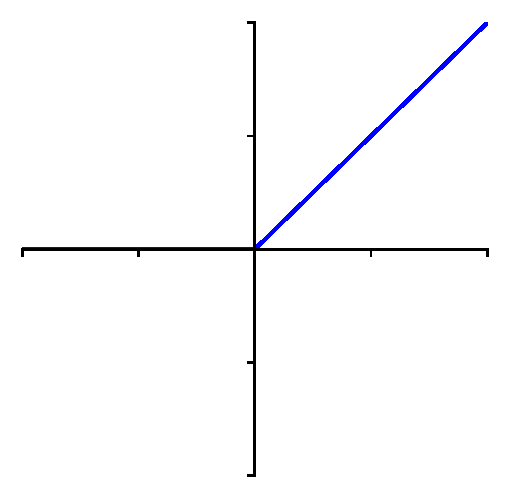
\includegraphics[width=6em]{figures/act-relu.pdf}\hspace*{3em}\includegraphics[width=6em]{figures/act-leaky-relu.pdf}\hspace*{3em}\includegraphics[width=6em]{figures/act-sigmoid.pdf}\\
        ``rectified linear unit (relu)'' \hspace*{1em} ``leaky relu'' \hspace*{4em} ``sigmoid'' \hspace*{4em}
      };
    \end{tikzpicture}
  \end{center}
\end{frame}


% Slide 13
\begin{frame}
  \frametitle{\vspace{-0.85cm}\begin{columns}\column{0.1\textwidth}\framebox{\includegraphics[width=\textwidth,trim = 30 20 10 10,clip]{figures/NN.pdf}}\column{0.85\textwidth}\vspace{-0.2cm}II.1: The Loss function quantifies our goal.\end{columns}}
  \tikzstyle{block} = [draw, text width=32em, fill=FERMILABblue!20, rounded corners, drop shadow, minimum height = 6em, align=left]
  \vspace*{-2em}
  \begin{center}
    \begin{tikzpicture}
      \node (loss) [block] at (0,0) {We have two choices:
        \begin{itemize}
        \item Kullback-Leibler (KL) divergence:\\
          $D_{KL} = \int p(x) \log \frac{p(x)}{q(x)} dx \qquad \approx \qquad \frac{1}{N} \sum \frac{p(x_{i})}{q(x_{i})} \log \frac{p(x_{i})}{q(x_{i})}, \qquad x_{i}\dots q(x)$
        \item Pearson $\chi^{2}$ divergence:\\
          $D_{\chi^{2}} = \int \frac{(p(x)-q(x))^{2}}{q(x)} dx\qquad \approx \qquad \frac{1}{N} \sum \frac{p(x_{i})^{2}}{q(x_{i})^{2}}-1, \qquad x_{i}\dots q(x)$
        \end{itemize}
      };
      \node (gradient) [block,anchor=north] at ($(loss.south)+(0em,-1em)$) {They give the gradient that is needed for the optimization:
        $$\nabla_{\theta} D_{(KL \text{ or } \chi^{2})} \approx - \frac{1}{N} \sum \left(\frac{p(x_{i})}{q(x_{i})}\right)^{(1  \text{ or } 2)}\nabla_{\theta} \log q(x_{i}), \qquad x_{i}\dots q(x)$$
      };
      \node (optimizer) [block,anchor=north] at ($(gradient.south)+(0em,-1em)$) {We use the ADAM optimizer for stochastic gradient descent:
        \begin{itemize}
        \item The learning rate for each parameter is adapted separately, but based on previous iterations.
        \item This is effective for sparse and noisy functions. 
        \end{itemize}
      };
      \node (ref) [text width = 20em,anchor = south east, align=right] at ($(optimizer.south east)+(0em,0em)$){\begin{scriptsize}\textcolor[rgb]{.4,.4,.4}{Kingma/Ba [arXiv:1412.6980]}\end{scriptsize}};
    \end{tikzpicture}
  \end{center}
\end{frame}


% Slide  14 (Sub-Mapping)
\begin{frame}
  \frametitle{Part II: \quad The Machine Learning approach}
  \vspace{0.5cm}
  \tikzstyle{partR} = [text width = 7cm,align=right]
  \tikzstyle{partL} = [text width = 7cm,align=left]
  \hspace*{-3em}
  \begin{tikzpicture}
    \node [partL](part1) at (0em,0em) {\large Part II.1: \quad Neural Network Basics};
    \node [anchor = west, text width = 6em](part1pic) at ($(part1.north east)+(1.5em,-0.75em)$) {\framebox{\includegraphics[width=8em,trim = 30 20 10 10,clip]{figures/NN.pdf}}};
    
    \node [partL, text width=20em,anchor=north] (part2) at ($(part1pic.south)+(0em,-3em)$) {\large Part II.2: \quad  Numerical Integration \\ with Neural Networks};
    \node [anchor = east, text width = 15em,align=left] (part2pic) at ($(part2.north west)+(0em,-0.75em)$) {\framebox{\includegraphics[width=14em]{figures/CL.png}}};
    
    \node [partL, align = right, text width = 8cm,anchor = north](part3) at ($(part2pic.south) + (0em,-4em)$) {\large Part II.3: \quad Examples};
    \node [anchor = west](part1pic) at ($(part3.north east)+(1.5em,-0.75em)$) {\framebox{\includegraphics[width=8em]{figures/3j_kin.png}}};
  \end{tikzpicture}
\end{frame}


\subsection{Part II.2: \quad Numerical Integration with Neural Networks}


% Slide 15
\begin{frame}
  \frametitle{\vspace{-0.85cm}\begin{columns}\column{0.1\textwidth}\framebox{\includegraphics[width=\textwidth,trim = 30 20 10 10,clip]{figures/NN.pdf}}\column{0.85\textwidth}\vspace{-0.2cm}II.2: Using the NN as coordinate transform is too costly.\end{columns}}
  \tikzstyle{block} = [draw, text width=32em, fill=FERMILABblue!20, rounded corners, drop shadow, minimum height = 6em, align=left]
  \vspace*{-2em}
  \begin{center}
    \begin{tikzpicture}
      \node (direct) [block] at (0,0) {We could use the NN as nonlinear coordinate transform:\vspace*{0.5em}
        \begin{itemize}
        \item We use a deep NN with $n_{dim}$ nodes in the first and last layer to map a uniformly distributed $x$ to a target $q(x)$.
        \item The distribution induced by the map $y(x)$ (=NN) is given by the Jacobian of the map:\\ $q(y) = q(y(x)) = \left|\frac{\partial y}{\partial x}\right|^{-1}$
        \end{itemize}
      };
      \node (plot0) [anchor=north, text width = 6em] at ($(direct.south)+(-5.5em,-0.5em)$) {\includegraphics[width=\textwidth]{figures/x2-map.pdf}};
      \node (plot1) [anchor=west, text width = 6em] at ($(plot0.east)+(5em,0em)$) {\includegraphics[width=\textwidth]{figures/x2-jac.pdf}};
      \node (arrow) [anchor = west, text width = 4em, text centered] at ($(plot0.east)+(0em,0em)$) {\begin{Large}$\xrightarrow{\text{Jacobian}}$\end{Large}};
      \node (ref) [text width = 20em,anchor = south east, align=right] at ($(direct.south east)+(0em,0em)$){\begin{scriptsize}\textcolor[rgb]{.4,.4,.4}{Klimek/Perelstein [arXiv:1810.11509]}\end{scriptsize}};
      \node (text0) [anchor=north, text width = 5em, text centered] at ($(plot0.south)+(0em,0.5em)$) {$y = x^{2}$};
      \node (text1) [anchor=north, text width = 6em, text centered] at ($(plot1.south)+(0em,0.5em)$) {$\left|\frac{\partial y}{\partial x}\right|^{-1} = \frac{1}{2x}$};
      \uncover<2->{\node (bad) [block,anchor=north, minimum height = 1em] at ($(direct.south)+(0em,-10em)$) {$\Rightarrow$ The Jacobian is needed to evaluate the loss, the integral, and to sample. However, it scales as $\mathcal{O}(n^{3})$ and is too costly for high-dimensional integrals!};
      }
    \end{tikzpicture}
  \end{center}
\end{frame}


% Slide 16 
\begin{frame}
  \frametitle{\vspace{-0.85cm}\begin{columns}\column{0.1\textwidth}\framebox{\includegraphics[width=\textwidth,trim = 30 20 10 10,clip]{figures/NN.pdf}}\column{0.85\textwidth}\vspace{-0.2cm}II.2: Normalizing Flows are numerically cheaper.\end{columns}}
  \tikzstyle{block} = [draw, text width=32em, fill=FERMILABblue!20, rounded corners, drop shadow, minimum height = 6em, align=left]
  \vspace*{-2em}
  \begin{center}
    \begin{tikzpicture}
      \node (NF) [block] at (0,0) {A Normalizing Flow:\\ \vspace*{0.5em}
        \begin{itemize}
        \item is a deterministic, bijective, smooth mapping between two statistical distributions.
        \item is composed of a series of easy transformations, the {\it ``Coupling Layers''.}
        \item is still flexible enough to learn complicated distributions. 
        \end{itemize}
        \vspace*{0.5em} $\Rightarrow$ The NN does not learn the transformation, but the parameters of a series of easy transformations. 
      };
      \uncover<2->{
        \node (refs) [block, anchor=north] at ($(NF.south)+(0em,-1em)$) {
          \begin{itemize}
          \item The idea was introduced as ``Nonlinear Independent Component Estimation'' (NICE) in \textcolor[rgb]{.4,.4,.4}{Dinh et al. \begin{scriptsize}[arXiv:1410.8516]\end{scriptsize}}.
          \item In \textcolor[rgb]{.4,.4,.4}{Rezende/Mohamed \begin{scriptsize}[arXiv:1505.05770]\end{scriptsize}}, Normalizing Flows were first discussed with planar and radial flows.
          \item Our approach follows the ideas of \textcolor[rgb]{.4,.4,.4}{M\"uller et al. \begin{scriptsize}[arXiv:1808.03856]\end{scriptsize}},\\
            but with the modifications of \textcolor[rgb]{.4,.4,.4}{Durkan et al. \begin{scriptsize}[arXiv:1906.04032]\end{scriptsize}}.
          \item Our code uses {\tt TensorFlow 2.0-beta}, \textcolor[rgb]{.4,.4,.4}{\begin{scriptsize}{\tt www.tensorflow.org}\end{scriptsize}}.
          \end{itemize}
        };}
    \end{tikzpicture}
  \end{center}
\end{frame}


% Slide 17
\begin{frame}
  \frametitle{\vspace{-0.85cm}\begin{columns}\column{0.1\textwidth}\framebox{\includegraphics[width=\textwidth,trim = 30 20 10 10,clip]{figures/NN.pdf}}\column{0.85\textwidth}\vspace{-0.2cm}II.2: The Coupling Layer is the fundamental Building Block.\end{columns}}
  \tikzstyle{block} = [draw, text width=32em, fill=FERMILABblue!20, rounded corners, drop shadow, minimum height = 10em, align=left]
  \vspace*{-2em}
  \begin{center}
    \begin{tikzpicture}
      \node (CL) [block] at (0,0) {
        \begin{tikzpicture}[background rectangle/.style={fill=white}, show background rectangle]
          \node (NN) [text width = 2em, minimum height = 7.5em, text centered] at ($(8em,0em)$) {NN};
          \node (perm) [anchor=south,text width = 4em, text centered,minimum height = 1em] at ($(20.5em,-0.75em)$) {permutation};
          \node (xa) [anchor = west,minimum height = 1em, text width = 1em, align = left] at ($(2em,4em)$) {$x_{A}$};
          \node (xb) [anchor = west,minimum height = 1em, text width = 1em, align = left] at ($(2em,-4em)$) {$x_{B}$};
          \node (y) [anchor=south east, minimum height = 1em, text width = 1em, text centered] at ($(17.75em,0em)$) {$y$};
          \node (x) [anchor=south west, minimum height = 1em, text width = 1em, text centered] at ($(-5em,0em)$) {$x$};
          \node (C)[anchor=south , minimum height = 1em, text width = 4em, text centered] at ($(NN.south)+(-1.1em,-1.15em)$) {$C(x_{B};m(x_{A}))$};
          \draw[thick,->] ($(-6em,0em)$) -- ($(-2em,0em)$);
          \draw[thick] ($(-2em,0em)$) -- ($(2em,4em)$);
          \draw[thick] ($(-2em,0em)$) -- ($(2em,-4em)$);
          \draw[thick] ($(4em,-4em)$) -- ($(4.75em,-4em)$);
          \draw[thick] ($(10.75em,-4em)$) -- ($(12em,-4em)$);
          \draw[thick] ($(4.75em,-5em)$) rectangle ($(10.75em,-3em)$);
          \draw[thick] ($(4em,4em)$) -- ($(12em,4em)$);
          \draw[thick] ($(12em,4em)$) --($(16em,0em)$);
          \draw[thick] ($(12em,-4em)$) --($(16em,0em)$);
          \draw[thick] ($(16em,0em)$) --($(18em,0em)$);
          \draw[thick] ($(18em,-1em)$) rectangle ($(24em,1em)$);
          \draw[thick,->]($(24em,0em)$) --($(25em,0em)$);
          \draw[thick] ($(7em,-1em)$) rectangle ($(9em,1em)$);
          \draw[thick,->] ($(8em,4em)$) -- ($(8em,1em)$);
          \draw[thick,->] ($(8em,-1em)$) -- ($(8em,-3.75em)$);
        \end{tikzpicture}
      };
      \node (exp) [block,anchor=north] at ($(CL.south)+(0em,-0.5em)$) {};
      \node (left) [anchor = north west, text width = 10em, align = left] at ($(exp.north west)$) {forward:\vspace*{-0.8em}\begin{align}\begin{aligned}\nonumber y_{A} &= x_{A} \\ y_{B,i}&=C(x_{B,i}; m(x_{A})) \end{aligned}\end{align}
        inverse:\vspace*{-0.8em}\begin{align}\begin{aligned}\nonumber x_{A} &= y_{A} \\ x_{B,i}&=C^{-1}(y_{B,i}; m(x_{A})) \end{aligned}\end{align}};
      \node (right) [anchor = north east, text width = 20em, align = left] at ($(exp.north east)$) {The $C$ are numerically cheap, invertible, and separable in $x_{B,i}$. \\ $ $\\
        Jacobian:\vspace*{-0.8em}\begin{align}\begin{aligned}\nonumber \left|\frac{\partial y}{\partial x}\right| &= \begin{vmatrix}1 & \frac{\partial C}{\partial x_{A}} \\ 0 & \frac{\partial C}{\partial x_{B}}\end{vmatrix} = \Pi_{i}\frac{\partial C(x_{B,i}; m(x_{A}))}{\partial x_{B,i}} \end{aligned}\end{align}
        \qquad \qquad$\Rightarrow \mathcal{O}(n)$
      };
    \end{tikzpicture}
  \end{center}
\end{frame}


% Slide 18
\begin{frame}
  \frametitle{\vspace{-0.85cm}\begin{columns}\column{0.1\textwidth}\framebox{\includegraphics[width=\textwidth,trim = 30 20 10 10,clip]{figures/NN.pdf}}\column{0.85\textwidth}\vspace{-0.2cm}II.2: The Coupling Function is a piecewise approximation to the cdf.\end{columns}}
  \tikzstyle{block} = [draw, text width=33em, fill=FERMILABblue!20, rounded corners, drop shadow, minimum height = 10em, align=left]
  \vspace*{-2em}
  \begin{center}
    \begin{tikzpicture}
      \node (pwlin) [block] at (0,0) {piecewise linear coupling function:\\ \vspace*{0.8em}
        \includegraphics[width=6em]{figures/pdf-pwlin.pdf}\hspace*{4em}\alt<1>{\includegraphics[width=6em]{figures/cdf-pwlin.pdf}}{\includegraphics[width=6em]{figures/cdf-pwlin-pt.pdf}} \\
        The NN predicts the pdf bin heights $Q_{i}$. 
      };
      \node (label) [anchor = north west, text width = 10em] at ($(pwlin.north west)+(4.5em,-2.5em)$) {\begin{scriptsize}pdf \hspace*{6em} cdf\end{scriptsize}};
      \node (ref) [text width = 20em,anchor = north east, align=right] at ($(pwlin.north east)+(0em,0em)$){\begin{scriptsize}\textcolor[rgb]{.4,.4,.4}{M\"uller et al. [arXiv:1808.03856]}\end{scriptsize}};
      \uncover<2->{
        \node (text1) [text width = 15em, anchor = north east, align = left] at ($(pwlin.north east)$) {\begin{align}\begin{aligned}\nonumber C &= \sum_{k=1}^{b-1} Q_{k} + \alpha Q_{b} \\ \alpha &= \tfrac{x-(b-1)w}{w} \\ \left|\frac{\partial C}{\partial x_{B}}\right| &= \Pi_{i} \tfrac{Q_{b_{i}}}{w}\end{aligned}\end{align}};}
      \uncover<3->{
        \node (pwrqs) [block,anchor=north] at ($(pwlin.south)+(0em,-0.5em)$) {rational quadratic spline coupling function:\\ \vspace*{0.8em}
          \includegraphics[width=6em]{figures/cdf-pwrqs-pt.pdf}\\ The NN predicts the cdf bin widths, heights, and derivatives that go in $a_{i} \& b_{i}$.};
        \node (label2) [anchor = north west, text width = 10em] at ($(pwrqs.north west)+(4.5em,-2.5em)$) {\begin{scriptsize}cdf\end{scriptsize}};
        \node (ref) [text width = 20em,anchor = north east, align=right] at ($(pwrqs.north east)+(0em,0em)$){\begin{scriptsize}\textcolor[rgb]{.4,.4,.4}{Durkan et al. [arXiv:1906.04032]\\ Gregory/Delbourgo [IMA Journal of Numerical Analysis, '82]}\end{scriptsize}};
        \node (rqsformula) [anchor = north east, text width = 25em] at ($(pwrqs.north east)+(0em,-3em)$) {\begin{columns}\column{0.5\textwidth}\begin{align}\begin{aligned}\nonumber C = \frac{a_{2} \alpha^{2} + a_{1} \alpha + a_{0}}{b_{2} \alpha^{2} + b_{1} \alpha + b_{0}}\end{aligned}\end{align}\column{0.5\textwidth} \begin{itemize}\item still rather easy \item more flexible\end{itemize}\end{columns}};
      }
    \end{tikzpicture}
  \end{center}
\end{frame}


% Slide 19
\begin{frame}
  \frametitle{\vspace{-0.85cm}\begin{columns}\column{0.1\textwidth}\framebox{\includegraphics[width=\textwidth,trim = 30 20 10 10,clip]{figures/NN.pdf}}\column{0.85\textwidth}\vspace{-0.2cm}II.2: We need $\mathcal{O}(\log{n})$ Coupling Layers.\end{columns}}
  \tikzstyle{block} = [draw, text width=32em, fill=FERMILABblue!20, rounded corners, drop shadow, minimum height = 10em, align=left]
  \vspace*{-2em}
  \begin{center}
    \begin{tikzpicture}
      \node (pwlin) [block] at (0,0) {How many Coupling Layers do we need?\vspace*{0.8em}
        \begin{itemize}
        \item Enough to learn all correlations between the variables.
        \item As few as possible to have a fast code.
        \item[$ $]
        \item This depends on the applied permutations and the $x_{A}-x_{B}$-splitting:\\ (pppttt)$\leftrightarrow$(tttppp) \quad {\it vs.} \quad (pppptt)$\leftrightarrow$(ppttpp)$\leftrightarrow$(ttpppp)
        \item[$ $]
        \item More pass-through dimensions (p) means more points required for accurate loss.
        \item Fewer pass-through dimensions means more CLs needed.
        \item[$ $]
        \item For $\# p \approx \# t$, we can prove: \framebox{$4 \leq \# CLs \leq 2\log_{2} n_{dim}$}
        \end{itemize}};
    \end{tikzpicture}
  \end{center}
\end{frame}


% Slide 20
\begin{frame}
  \frametitle{\vspace{-0.85cm}\begin{columns}\column{0.1\textwidth}\framebox{\includegraphics[width=\textwidth,trim = 30 20 10 10,clip]{figures/NN.pdf}}\column{0.85\textwidth}\vspace{-0.2cm}II.2: We utilize different NN architectures.\end{columns}}
  \tikzstyle{block} = [draw, text width=32em, fill=FERMILABblue!20, rounded corners, drop shadow, minimum height = 10em, align=left]
  \vspace*{-2em}
  \begin{center}
    \begin{tikzpicture}
      \node (DNN) [block] at (0,0) {Available Architectures:\\
        \begin{columns}\column{0.5\textwidth}``Fully Connected'' Neural Net (NN):\\ \centering\framebox{\includegraphics[width=0.58\textwidth]{figures/DNN.pdf}}\column{0.5\textwidth}``U-shaped'' Neural Net (Unet): \\ \centering\framebox{\includegraphics[width=0.58\textwidth]{figures/UNN.pdf}} \end{columns}
      };
      \node (ref1) [text width = 20em,anchor = north east, align=right] at ($(DNN.north east)+(0em,0em)$){\begin{scriptsize}\textcolor[rgb]{.4,.4,.4}{M\"uller et al. [arXiv:1808.03856]}\end{scriptsize}};
      \uncover<2->{
        \node (Input) [block,anchor=north] at ($(DNN.south)+(0em,-0.5em)$) {There are different ways to encode the input dimensions $x_{A}$.\\ For example $x_{A} = (0.2,0.7)$:\vspace*{0.5em}
          \begin{itemize}
          \item direct: $x_{i} = (0.2,0.7)$
          \item one-hot (8 bins): $x_{i} = ((0,1,0,0,0,0,0,0),(0,0,0,0,0,1,0,0))$
          \item one-blob (8 bins): $x_{i} = ((0.55, 0.99, 0.67, 0.16, 0.01, 0, 0, 0)$, \hspace*{10em}$(0,0,0.01,0.11,0.55,0.99,0.67,0.16))$
            \vspace*{0.5em}
          \end{itemize}
        };
        \node (ref2) [text width = 20em,anchor = south east, align=right] at ($(Input.south east)+(0em,0em)$){\begin{scriptsize}\textcolor[rgb]{.4,.4,.4}{M\"uller et al. [arXiv:1808.03856]}\end{scriptsize}};}
    \end{tikzpicture}
  \end{center}
\end{frame}


% Slide  21 (Sub-Mapping)
\begin{frame}
  \frametitle{Part II: \quad The Machine Learning approach}
  \vspace{0.5cm}
  \tikzstyle{partR} = [text width = 7cm,align=right]
  \tikzstyle{partL} = [text width = 7cm,align=left]
  \hspace*{-3em}
  \begin{tikzpicture}
    \node [partL](part1) at (0em,0em) {\large Part II.1: \quad Neural Network Basics};
    \node [anchor = west, text width = 6em](part1pic) at ($(part1.north east)+(1.5em,-0.75em)$) {\framebox{\includegraphics[width=8em,trim = 30 20 10 10,clip]{figures/NN.pdf}}};
    
    \node [partL, text width=20em,anchor=north] (part2) at ($(part1pic.south)+(0em,-3em)$) {\large Part II.2: \quad  Numerical Integration \\ with Neural Networks};
    \node [anchor = east, text width = 15em,align=left] (part2pic) at ($(part2.north west)+(0em,-0.75em)$) {\framebox{\includegraphics[width=14em]{figures/CL.png}}};
    
    \node [partL, align = right, text width = 8cm,anchor = north](part3) at ($(part2pic.south) + (0em,-4em)$) {\large Part II.3: \quad Examples};
    \node [anchor = west](part1pic) at ($(part3.north east)+(1.5em,-0.75em)$) {\framebox{\includegraphics[width=8em]{figures/3j_kin.png}}};
  \end{tikzpicture}
\end{frame}


\subsection{Part II.3: \quad Examples}


% Slide 22
\begin{frame}
  \frametitle{\vspace{-0.85cm}\begin{columns}\column{0.1\textwidth}\framebox{\includegraphics[width=\textwidth,trim = 30 20 10 10,clip]{figures/NN.pdf}}\column{0.85\textwidth}\vspace{-0.2cm}II.3: The 4-d Camel function illustrates the learning of the NN.\end{columns}}
  \tikzstyle{block} = [draw, text width=32em, fill=FERMILABblue!20, rounded corners, drop shadow, minimum height = 4em, align=left]
  \vspace*{-2em}
  \begin{center}
    \begin{tikzpicture}
      \node (func) [block] at (0,0) {Our test function: 2 Gaussian peaks, randomly placed in a 4d space.\vspace*{0.5em}
        \begin{columns}\column{0.5\textwidth}\hspace*{1.25em} Target Distribution:\\ \centering\framebox{\includegraphics[width=0.75\textwidth]{code/matrix.png}}\column{0.5\textwidth}
          \only<1>{Before training: \\ \centering\framebox{\includegraphics[width=0.75\textwidth]{code/fig-0000.png}} \end{columns}}
        \only<2>{After 5 epochs: \\ \centering\framebox{\includegraphics[width=0.75\textwidth]{code/fig-0005.png}} \end{columns}}
      \only<3>{After 10 epochs: \\ \centering\framebox{\includegraphics[width=0.75\textwidth]{code/fig-0010.png}} \end{columns}}
    \only<4>{After 25 epochs: \\ \centering\framebox{\includegraphics[width=0.75\textwidth]{code/fig-0025.png}} \end{columns}}
  \only<5>{After 100 epochs: \\ \centering\framebox{\includegraphics[width=0.75\textwidth]{code/fig-0100.png}} \end{columns}}
\only<6>{After 200 epochs: \\ \centering\framebox{\includegraphics[width=0.75\textwidth]{code/fig-0199.png}} \end{columns}}
};
\node (gif) [block,anchor=north] at ($(func.south)+(0em,-0.5em)$) {\vspace*{-0.25em}
  \begin{itemize}
  \item Final Integral:    0.0063339(41)
  \item {\tt VEGAS} plain: 0.0063349(92)
  \item {\tt VEGAS} full:  0.0063326(21)
  \item Trained efficiency: 14.8 \% \qquad Untrained efficiency: 0.6 \%
  \end{itemize}
  % \animategraphics[loop,controls,width=12em]{10}{code/fig-}{0000}{0199}
};
\end{tikzpicture}
\end{center}
\end{frame}


% Slide 23
\begin{frame}
  \frametitle{\vspace{-0.85cm}\begin{columns}\column{0.1\textwidth}\framebox{\includegraphics[width=\textwidth,trim = 30 20 10 10,clip]{figures/NN.pdf}}\column{0.85\textwidth}\vspace{-0.2cm}II.3: Sherpa needs a high-dimensional integrator.\end{columns}}
  \tikzstyle{block} = [draw, text width=32em, fill=FERMILABblue!20, rounded corners, drop shadow, minimum height = 10em, align=left]
  \vspace*{-2em}
  \begin{center}
    \begin{tikzpicture}
      \node (sherpa) [block] at (0,0) {Sherpa is a Monte Carlo event generator for the {\bf S}imulation of {\bf H}igh-{\bf E}nergy {\bf R}eactions of {\bf PA}rticles. We use Sherpa to \vspace*{0.5em}
        \begin{itemize}
        \item map the unit-hypercube of our integration domain to momenta and angles. To improve efficiency, Sherpa uses a recursive multichannel algorithm.
        \item[$\Rightarrow$] $n_{dim} = \underbrace{3 n_{final} -4}_{\text{kinematics}} + \underbrace{n_{final}-1}_{{\text{multichannel}}} $
        \item compute the matrix element of the process. The {\tt COMIX++} ME-generator uses color-sampling, so we need to integrate over final state color configurations, too.  
        \end{itemize}
        \vspace*{0.5em}
        \begin{center}
          \framebox{$\Rightarrow n_{dim} = 4 n_{final} -3 + 2(n_{color})$}
        \end{center}
        $ $
      };
      \node (ref) [text width = 20em,anchor = south east, align=right] at ($(sherpa.south east)+(0em,0em)$){\begin{scriptsize}\textcolor[rgb]{.4,.4,.4}{      https://sherpa.hepforge.org/}\end{scriptsize}};
    \end{tikzpicture}
  \end{center}
\end{frame}


% Slide 23
\begin{frame}
  \frametitle{\vspace{-0.85cm}\begin{columns}\column{0.1\textwidth}\framebox{\includegraphics[width=\textwidth,trim = 30 20 10 10,clip]{figures/NN.pdf}}\column{0.85\textwidth}\vspace{-0.2cm}II.3: Already in $e^{+}e^{-}\to 3j$ we are more effective.\end{columns}}
  \tikzstyle{block} = [text width=22em, minimum height = 10em, align=left]
  \tikzstyle{label} = [text width = 18em,align = left, anchor = west]
  \vspace*{-2em}
  \begin{center}
    \begin{tikzpicture}
      \node (plot) [block] at (0,0) {\includegraphics[width=\textwidth]{figures/3j-matrix.png}
      };
      \node (l1) [label] at ($(-8em,10em)$) {$\leftarrow$ spectator of $q$ color};
      \node (l2) [label] at ($(-6.3em,8.3em)$) {$\leftarrow$ $q$ color};
      \node (l3) [label] at ($(-4.7em,6.7em)$) {$\leftarrow$ spectator of $g$ color};
      \node (l4) [label] at ($(-3em,5em)$) {$\leftarrow$ $g$ color};
      \node (l5) [label] at ($(-1.4em,3.4em)$) {$\leftarrow$ propagator of decaying fermion};
      \node (l6) [label] at ($(0.2em,1.8em)$) {$\leftarrow$ $\cos \vartheta$ of decaying fermion with beam};
      \node (l7) [label] at ($(1.8em,0.2em)$) {$\leftarrow$ $ \varphi$ of decaying fermion with beam};
      \node (l8) [label] at ($(3.4em,-1.4em)$) {$\leftarrow$ $\cos \vartheta$ of decay};
      \node (l9) [label] at ($(5em,-3em)$) {$\leftarrow$ $ \varphi$ of decay};
      \node (l10) [label,text width = 10em] at ($(12em,-7em)$) {$\leftarrow$  multichannel};
      \node (headline) [anchor = north east, text width = 15em, align=right] at ($(15em,10em)$) {\framebox{Target distribution}};
    \end{tikzpicture}
  \end{center}
\end{frame}


% Slide 25 
\begin{frame}
  \frametitle{\vspace{-0.85cm}\begin{columns}\column{0.1\textwidth}\framebox{\includegraphics[width=\textwidth,trim = 30 20 10 10,clip]{figures/NN.pdf}}\column{0.85\textwidth}\vspace{-0.2cm}II.3: Already in $e^{+}e^{-}\to 3j$ we are more effective.\end{columns}}
  \tikzstyle{block} = [text width=22em, minimum height = 10em, align=left]
  \tikzstyle{label} = [text width = 18em,align = left, anchor = west]
  \vspace*{-2em}
  \begin{center}
    \begin{tikzpicture}
      \node (plot) [block] at (0,0) {\includegraphics[width=\textwidth]{figures/3j-matrix-learned.png}
      };
      \node (l1) [label] at ($(-8em,10em)$) {$\leftarrow$ spectator of $q$ color};
      \node (l2) [label] at ($(-6.3em,8.3em)$) {$\leftarrow$ $q$ color};
      \node (l3) [label] at ($(-4.7em,6.7em)$) {$\leftarrow$ spectator of $g$ color};
      \node (l4) [label] at ($(-3em,5em)$) {$\leftarrow$ $g$ color};
      \node (l5) [label] at ($(-1.4em,3.4em)$) {$\leftarrow$ propagator of decaying fermion};
      \node (l6) [label] at ($(0.2em,1.8em)$) {$\leftarrow$ $\cos \vartheta$ of decaying fermion with beam};
      \node (l7) [label] at ($(1.8em,0.2em)$) {$\leftarrow$ $ \varphi$ of decaying fermion with beam};
      \node (l8) [label] at ($(3.4em,-1.4em)$) {$\leftarrow$ $\cos \vartheta$ of decay};
      \node (l9) [label] at ($(5em,-3em)$) {$\leftarrow$ $ \varphi$ of decay};
      \node (l10) [label,text width = 10em] at ($(12em,-7em)$) {$\leftarrow$  multichannel};
      \node (headline) [anchor = north east, text width = 15em, align=right] at ($(15em,10em)$) {\framebox{Learned distribution}};
    \end{tikzpicture}
  \end{center}
\end{frame}


% Slide 26
\begin{frame}
  \frametitle{\vspace{-0.85cm}\begin{columns}\column{0.1\textwidth}\framebox{\includegraphics[width=\textwidth,trim = 30 20 10 10,clip]{figures/NN.pdf}}\column{0.85\textwidth}\vspace{-0.2cm}II.3: Already in $e^{+}e^{-}\to 3j$ we are more effective.\end{columns}}
  \tikzstyle{block} = [draw, text width=32em, fill=FERMILABblue!20, rounded corners, drop shadow, minimum height = 2em, align=left]
  \vspace*{-2em}
  \begin{center}
    \begin{tikzpicture}
      \node (plot) [block] at (0,0) {
        \begin{center}
          \includegraphics[width=0.75\textwidth]{code/weights/weights.pdf}
        \end{center}
      };
      \node (text) [block,anchor=north] at ($(plot.south)+(0em,-1em)$) {\vspace*{-1em}
        \begin{align}\begin{aligned}\nonumber \sigma_{\text{our code}} = 4887.1 \pm 4.6 \text{pb} \hspace*{6em} \sigma_{\text{Sherpa}} = 4877.0 \pm 17.7 \text{pb} \\ \text{unweighting efficiency} = 12.9 \% \hspace*{4em}\text{unweighting efficiency} = 2.8 \% \end{aligned}\end{align}
        % xsec = 4887.097353541995 +/- 4.556917423148081 12.9 \%
        % 4877.01 pb +- ( 17.7023 pb = 0.36 \% ) exp. eff: 2.78364 \%
      };
      \node [anchor = north, text width = 22em, align = left] (label) at ($(plot.north)+(0em,-1em)$) {weight distribution};
    \end{tikzpicture}
  \end{center}
\end{frame}


% Slide 27
\begin{frame}
  \frametitle{Improving Numerical Integration and Event Generation with Normalizing Flows}% \\ --- Summary ---}
  \vspace*{-0.25em}
  \tikzstyle{summary} = [draw, text width=32em, fill=FERMILABblue!20, rounded corners, drop shadow,minimum height=6.75em]
  \begin{center}
    \begin{tikzpicture}
      \node (con1) [summary] at (0,0) {};
      \node (pic1) [anchor=east] at ($(con1.east)$) {\framebox{\includegraphics[width=6em,trim = 30 20 10 10,clip]{figures/NN.pdf}}};
      \node (sum1) [anchor=west,text width = 25em] at ($(con1.west)+(-0.75em,0.25em)$) {\begin{itemize}
        \item I summarized the concepts of numerical integration and the ``traditional'' VEGAS algorithm. 
          % \item[$ $]
        \item I introduced Neural Networks as versatile nonlinear functions. 
        \end{itemize}};
      \uncover<2->{
        \node (con2) [summary,anchor=north] at ($(con1.south)+(0em,-0.6em)$) {};
        \node (pic2) [anchor=east] at ($(con2.east)$) {\framebox{\includegraphics[width=14em]{figures/CL.png}}};
        \node (sum2) [anchor=west,text width = 15em] at ($(con2.west)+(-0.75em,0.25em)$) {\begin{itemize}
          \item I presented the idea of Normalizing Flows. 
            % \item[$ $]
          \item  I discussed their superiority for large integration dimensions.
          \end{itemize}};
      }
      \uncover<3->{
        \node (con3) [summary,anchor=north] at ($(con2.south)+(0em,-0.6em)$) {};
        \node (pic3) [anchor=east] at ($(con3.east)$) {\framebox{\includegraphics[width=5em]{figures/3j_kin.png}}};
        \node (sum3) [anchor=west,text width = 32em] at ($(con3.west)+(-0.75em,0.25em)$) {\begin{itemize}
          \item I showed the results of two different examples
          \item In $e^{+}e^{-}\to 3j$, we ``beat'' Sherpa by roughly a factor of 5.
          \end{itemize}};
      }
    \end{tikzpicture}
  \end{center}
\end{frame}


%%%\section*{Backup}
%%%\addtocounter{framenumber}{-1} 
%%%\begin{frame}
%%%  \begin{center}
%%%    {\Huge Backup}
%%%  \end{center}
%%%\end{frame}

%%%%%
%%%%%\addtocounter{framenumber}{-1} 
%%%%%\begin{frame}
%%%%%  \frametitle{ }
%%%%%\end{frame}
\end{document}









